%%%%%%%%%%%%%%%%%%%%%%%%%%%%%%%%%%%%%%
%%%%%%%%%%%%%%%%%%%%%%%%%%%%%%%%%%%%%%
% Do not edit the TeX file your work
% will be overwritten.  Edit the RnW
% file instead.
%%%%%%%%%%%%%%%%%%%%%%%%%%%%%%%%%%%%%%
%%%%%%%%%%%%%%%%%%%%%%%%%%%%%%%%%%%%%%




We next consider functional perturbations to the prior on the sticks. \prettyref{fig:functional_sens_plot_thresh0} shows the effect of our choice of $\phi$ on the expected number of distinct clusters ($t = 0$). Both the in-sample and the predictive quantities are displayed. The approximation is most accurate at small $\epsilon$, though the predictive quantity for the first perturbation was fairly accurate for the entire range of $\epsilon \in [0, 1]$. 



\begin{knitrout}
\definecolor{shadecolor}{rgb}{0.969, 0.969, 0.969}\color{fgcolor}\begin{figure}[!h]

{\centering 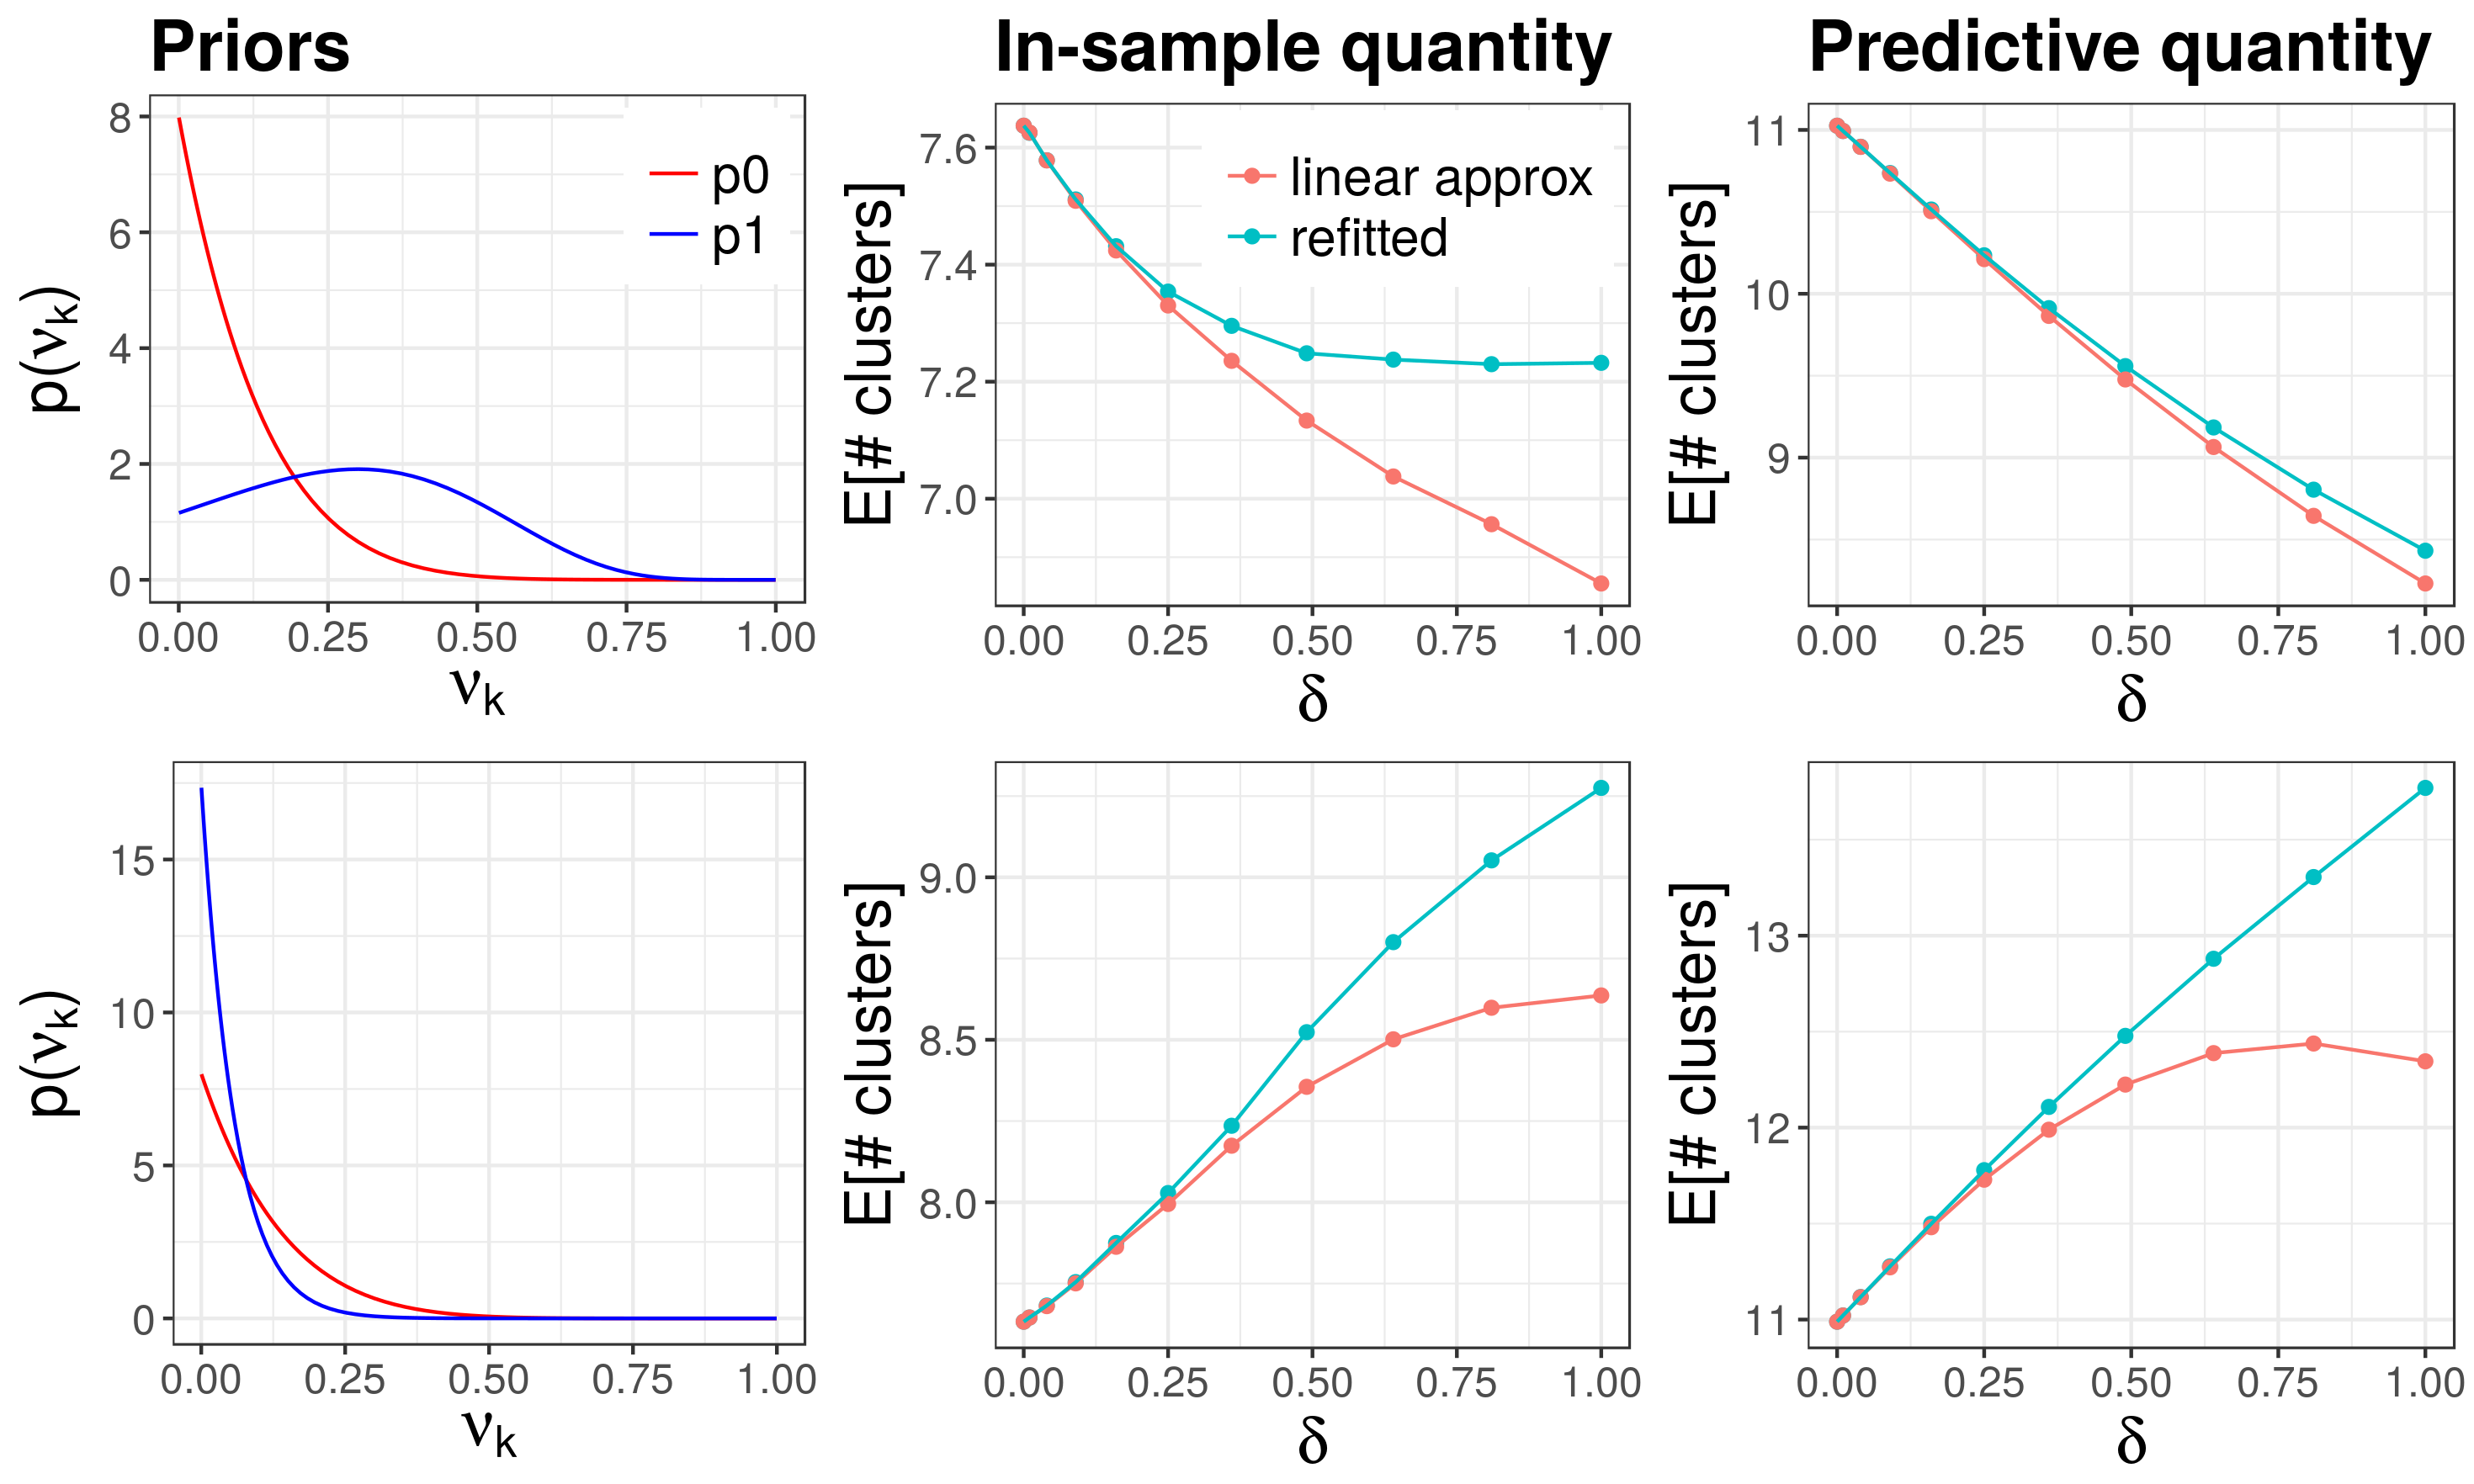
\includegraphics[width=0.98\linewidth,height=0.588\linewidth]{figure/functional_sens_plot_thresh0-1} 

}

\caption{\label{fig:func_sens_e_num_clusters_thresh0}
The effect of prior perturbation on the expected number of distinct clusters ($t = 0$). 
Left column: the original prior $p_{0}$ in red,
the perturbed prior $p_c$ in blue. 
Middle: linearly approximated vs.
re-fitted in-sample expected number of clusters. 
Right: linearly approximated vs.
re-fitted predictive expected number of clusters.  }\label{fig:functional_sens_plot_thresh0}
\end{figure}


\end{knitrout}
%
Finally, we consider the same functional perturbation to the stick priors, but with the threshold for counting a cluster at $t = 3$. \prettyref{fig:functional_sens_plot_thresh0} displays the comparison of the linear approximation against the refitted values, for both the in-sample and the predictive quantities. In this case, the choice of perturbation did not significantly move the number of thresholded clusters in the re-fitted values. 



\begin{knitrout}
\definecolor{shadecolor}{rgb}{0.969, 0.969, 0.969}\color{fgcolor}\begin{figure}[!h]

{\centering \includegraphics[width=0.98\linewidth,height=0.588\linewidth]{figure/functional_sens_plot_thresh3-1} 

}

\caption{\label{fig:func_sens_e_num_clusters_thresh3}
The effect of prior perturbation on the expected number of clusters with at least three 
data points ($t = 3$). 
Left column: the original prior $p_{0}$ in red,
the perturbed prior $p_c$ in blue. 
Middle: linearly approximated vs.
re-fitted in-sample expected number of clusters. 
Right: linearly approximated vs.
re-fitted predictive expected number of clusters.  }\label{fig:functional_sens_plot_thresh3}
\end{figure}


\end{knitrout}
